\documentclass[a4,12pt]{article}
\usepackage[utf8]{inputenc}
\usepackage[spanish]{babel}
\usepackage[margin=3cm]{geometry}
\usepackage{graphicx}
\usepackage{import}
\usepackage{color}
\usepackage{verbatim}
\usepackage{listings}
\usepackage[normalem]{ulem}

\usepackage[hidelinks]{hyperref}

\title{Comparación de Algoritmos de Ordenación}
\author{Vicente Javier Vidal-Abarca González}
\date{12 de junio de 2017}

\begin{document}

\maketitle

\begin{abstract}

Este documento, ha sido creado en \LaTeX, con el fin mostrar el conocimiento que poseo para crear un documento con dicha herramienta. Además, de guardar un registro de control usando GIT. Para demostrarlo, voy a realizar un pequeño codigo en python, que comparará el tiempo que tarda en ordenar una lista de un tamaño predefinido, usando tanto el algoritmo de Burbuja, como el Quicksort.

\end{abstract}

\newpage
\tableofcontents
\newpage

\section{Introducción}
Bienvenido a este documento. Como bien esta explicado en el resumen, este documento ha sido realizado en \LaTeX, y con el mostraré el desarrollo de esta práctica.

\subsection{Programas usados}
En esta práctica, he usado 3 programas principalmente:
\begin{itemize}

\item GIT: Repositorio usado para almacenar las pruebas de control de la práctica.

\item \LaTeX: Herramienta usada para crear este documento PDF eficientemente.

\item Python IDLE: Entorno donde he desarrollado el código y las pruebas necesarias para realizar este proyecto.

\end{itemize}

\newpage
\section{GIT}
Aquí se explicará los comandos mas utilizados, y como he planteado el desarrollo de este documento haciendo uso del control proporcionado por GIT.

\subsection{git init}
Usando el comando \texttt{git init <carpeta>} preparamos una carpeta con un proyecto de git vacío para comenzar a usar GIT.

\bigskip
En mi caso, he usado una carpeta nombrada por el nombre de ``DIS''.

\subsection{git add}
Usando el comando \texttt{git add <fichero>} añadimos ficheros al "index" (también conocido como HEAD). En este index, se hace una "previa" de como se encontrará la carpeta cuando hagamos un guardado real, usando el comando que se explicará mas adelante de \texttt{git commit}.

\subsection{git commit}
Usando el comando \texttt{git commit -m ``Mensaje del commit"}, se realizan los cambios definitivamente en el repositorio de GIT. Con el parámetro -m, introducimos un pequeño texto para tener una orientación de que ha realizado dicho guardado.

\subsection{git checkout}
El comando \texttt{git checkout}, sirve para cambiar entre distintas ramas del proyecto.

\bigskip
Además, también sirve para crear ramas usando \texttt{git checkout -b <nueva\_rama>}, o bien para borrarlas con \texttt{git checkout -d <rama\_a\_borrar>}.

\subsection{git log}
El comando \texttt{git log} muestra un pequeño resumen de los commits que han sido emitidos en la rama en la que te encuentres.

\subsection{git status}
El comando \texttt{git status} muestra el estado de los archivos que hay en la rama en la que te encuentres. Especifica si un archivo ha sido borrado, añadido o modificado desde el último commit realizado en esa misma rama.

\subsection{gitg}
Este comando lo usamos en el laboratorio de prácticas, y sirve para poder comprobar gráficamente como se encuentra el proyecto de GIT. Que ramas tiene, que archivos tiene cada rama, etc. Además de esto, también se puede hacer desde la herramienta gráfica los commits y otros comandos de GIT.

\bigskip
Sin embargo, yo no he podido usar esta herramienta gráfica, y por lo tanto he usado un repositorio remoto de github, creado especificamente para esto. Para realizar dicho repositorio:

\subsubsection{GitHub}
Primero, en la página de \texttt{github.com} he creado una cuenta (con nombre de usuario karatekav), y he creado un repositorio con el mismo nombre que tiene la carpeta que uso GIT, es decir, DIS.

\subsubsection{Añadir el repositorio remoto}
Una vez creado el repositorio, he añadido a la carpeta este mismo. Esto ha sido con el uso de: 

\noindent\texttt{git remote add origin https://github.com/<nombre\_usuario>/<nombre\_rep>.git} 

Que en mi caso específico ha sido: 

\noindent\texttt{git remote add origin https://github.com/karatekav/DIS.git}.

\subsubsection{Guardar en el repositorio remoto}
Para guardar en el repositorio añadido como \texttt{origin}, es tan simple como realizar el comando de git push. Para ello:

\noindent\texttt{git push origin <rama\_a\_guardar>}.

Como la rama principal es master, la mayoría de guardados se realizaran con el siguiente comando:

\noindent\texttt{git push origin master}.

\subsection{Otros}
Además, he creado el archivo \texttt{.gitignore} para no guardar en GIT los archivos que son necesarios para la creación del PDF autogenerados por el compilador de \LaTeX .

\newpage

\section{\LaTeX}

En esta sección explicaré a grandes rasgos las cosas que más he utilizado en \LaTeX.

\bigskip
He usado \verb+\maketitle+ con los parámetros de \verb+\title+, \verb+\author+ y \verb+\date+ para crear la primera parte de este documento.

\bigskip
Además para poner todos estos comandos de \LaTeX, estoy usando \verb+\verb+. Si es para poner un comando de otras herramientas como GIT, he usado el comando de \verb+\texttt{<comando>}+.

\bigskip
Con esto mencionado, y usando el bloque de \verb+\begin{abstract} <resumen> \end{abstract}+, se crea el pequeño resumen que también se encuentra en la primera página de este documento.

\bigskip
Uso \verb+\tableofcontents+ para crear el índice. Además, he incluido el paquete \texttt{hiperref}, usando \verb+[hidelinks]+ para quitar el enlace en color rojo.

\bigskip
En general, uso \verb+\newpage+ para introducir un salto de página y \verb+\bigskip+ para crear una línea en blanco entre párrafos distintos, como se puede ver en esta parte del documento.

\bigskip
Uso los comandos de \verb+\section{<nombre_sección>}+, \verb+\subsection{nombre_subsección}+ y \verb+\subsubsection{nombre_subsubsección}+ para crear los apartados que funcionarán con el índice.

\bigskip
Además de eso, para crear un apartado de una lista de objetos, usaremos la siguiente estructura:
\verb+\begin{itemize} \item <Nombre_item> \end{itemize}+, donde cada \verb+\item <Nombre_item>+ corresponde a una nueva línea que tendŕa la lista. 

Un ejemplo realizado en este documento es en el apartado de introducción, cuando se especifican las 3 herramientas principales usadas en esta práctica.

\bigskip
Además de estos comandos principales, quiero destacar el uso de herramientas externas (make con F12), y snippets que he ido personalizando, y que son muy útiles para este desarrollo. Por ejemplo, un snippet que es ``sk'', que al usarlo se transforma en \verb+\bigskip+.

\newpage
\section{Python IDLE}
Python IDLE es el entorno donde he desarrollado el código en python donde voy a comparar los dos algoritmos de ordenación.

\bigskip
\noindent Los dos algoritmos que he utilizado son:
\begin{enumerate}

\item \textbf{Burbuja}: Revisa cada elemento de la lista que va a ser ordenada con el siguiente, intercambiándolos de posición si están en el orden equivocado.

\item \textbf{Quicksort}: Se basa en el algoritmo de divide y vencerás. Se basa en dividir el problema en dos mitades iguales, y hacer llamadas recursivas a si misma con cada una de estas partes, hasta llegar a un problema tan pequeño que sea directo.
\end{enumerate}

\noindent Para comprobar la potencia de estos algoritmos, se crea una lista aleatoria de números, de 0 a n-1. Siendo n el número total de elementos de la lista.

\bigskip
Como tamaños de entrada (el número n comentado anteriormente), tenemos los siguientes:

500, 1000, 2000, 5000, 10000, 20000, 30000, 40000 y 50000.

\bigskip
Por último, usando la librería de python \texttt{matplotlib}, pintaré una gráfica de los resultados en tiempo obtenidos, usando la función time de la librería \texttt{time} de pyhton.

\begin{center}
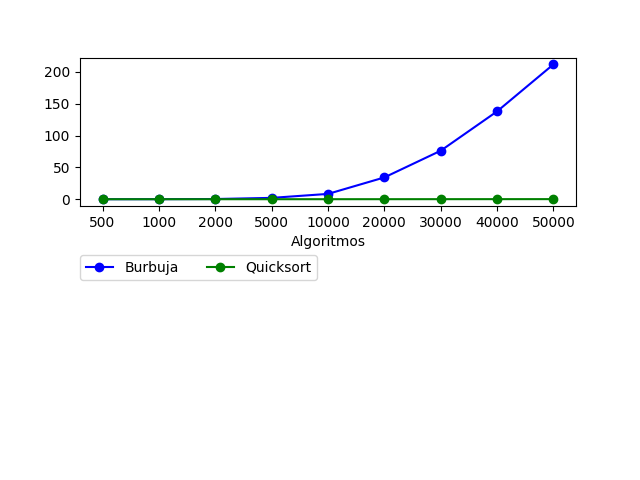
\includegraphics[width=1\textwidth]{Comparativa/Comparacion.png}
\end{center}

\newpage
\section{Conclusión}
La herramienta de \LaTeX es bastante útil y con más experiencia y mucha práctica se pueden generar muy buenos documentos PDFs, y muy rápido.

Cabe destacar, que funciones del gedit aprendidas en clase, como por ejemplo los snippets y las external tools de gedit, son muy muy útiles y un gran descubrimiento para el desarrollo de cualquier proyecto.

\bigskip
Ahora debería de mostrar la bibliografía incluida en el fichero \texttt{bibliografia.bib}, pero por algún motivo no se muestra correctamente.
\bibliography{bibliografia}{}
\bibliographystyle{plain}

\end{document}
